\documentclass{standalone}
\usepackage{tikz}
\usepackage[siunitx, RPvoltages]{circuitikzgit}
%\usepackage[]{circuitikz}

\usetikzlibrary{positioning, arrows, shapes.gates.logic.US, shapes.gates.logic.IEC, calc}

\begin{document}

\resizebox{10cm}{5cm}{


    \ctikzset{
        logic ports=ieee,
        logic ports/scale=0.7,
     }
     
    \tikzset{sr-ff/.style={flipflop, flipflop def={
        t1=S,
        t2=CP,
        t3=R,
        t4={\ctikztextnot{Q}},
        t6=Q,
        nd=1}},
    }
    
    \begin{circuitikz}[]
        \draw (0,0) node[sr-ff](FF){} (FF.bup)
            node[above]{SR-FF};
        \draw (FF.pin 1) -- ++(-1,0) node[and port,
            anchor=out](AND1){}
            (FF.pin 3) -- ++(-1,0) node[and port,
            anchor=out](AND2){};
    \end{circuitikz}

    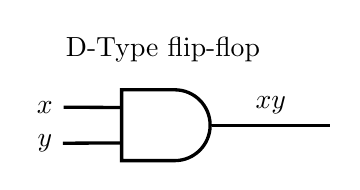
\begin{tikzpicture}[node distance=.2cm, label distance=2mm, very thick]

        %INPUTS
        \node[] (x) at (0,.46) {\normalsize $x$};
        \node[] (y) at (0,0)   {\normalsize $y$};

        % AND (NOTE I'M USING 3 INPUTS)
        \node[and gate US, draw, rotate=0, logic gate inputs=nnn] (AND) at ($(y) + (1.5,.23)$) {};
        \draw (x) -- (AND.input 1);
        \draw (y) -- (AND.input 3);
        \draw (AND.output) -- node[above]{\normalsize $xy$} ([xshift=1.5cm]AND.output);
        \node[above=of AND] {\normalsize D-Type flip-flop};

    \end{tikzpicture}
}

\end{document} 
